\documentclass{article}

\usepackage{amsmath, amsthm, amssymb, amsfonts}
\usepackage{thmtools}
\usepackage{graphicx}
\usepackage{setspace}
\usepackage{geometry}
\usepackage{float}
\usepackage{hyperref}
\usepackage[utf8]{inputenc}
\usepackage[english]{babel}
\usepackage{framed}
\usepackage[dvipsnames]{xcolor}
\usepackage{tcolorbox}
\usepackage{enumitem}
\usepackage{tikz}
\usepackage{tikz-3dplot}
\usepackage{graphicx}

% \colorlet{LightGray}{White!90!Periwinkle}
\colorlet{LightGray}{Blue!30}
\colorlet{LightOrange}{Orange!15}
\colorlet{LightGreen}{Green!15}

\newcommand{\HRule}[1]{\rule{\linewidth}{#1}}

\declaretheoremstyle[name=Theorem,]{thmsty}
\declaretheorem[style=thmsty,numberwithin=section]{theorem}
\tcolorboxenvironment{theorem}{colback=LightGray}

\declaretheoremstyle[name=Proposition,]{prosty}
\declaretheorem[style=prosty,numberlike=theorem]{proposition}
\tcolorboxenvironment{proposition}{colback=LightOrange}

\declaretheoremstyle[name=Principle,]{prcpsty}
\declaretheorem[style=prcpsty,numberlike=theorem]{principle}
\tcolorboxenvironment{principle}{colback=LightGreen}


\makeatletter
\renewcommand{\maketitle}{%
  \begin{center}
    \vspace*{3cm} % Adjust the vertical space as needed
    {\LARGE\@author\par}
    \vspace{1cm} % Adjust the vertical space as needed
    {\Huge\bfseries\@title\par}
    \vspace{2cm} % Adjust the vertical space as needed
    {\Large\@date\par}
  \end{center}
}
\makeatother


\begin{document}

\title{ \normalsize \textsc{}
\\ [0.5cm]
\HRule{1.0pt} \\
\Huge \textbf{The Evasion Problem}
\HRule{1.0pt}
\\ [1.5cm]
\LARGE{Andrej Jočić \\ Matija Ojo}
}
\author{\textbf{Computational Topology - group project}}
\date{\today}

\maketitle

\newpage


\section{Introduction}

The evasion problem asks if there is a way to move in an area, covered with moving sensors, and not be detected.
We assume the sesnors follow a predefined path and their movement is periodic.
This means that, after some period, the area covered by sesnors is identical.
Furthermore, we assume the area in question is a subspace of the plane $ \mathbb{R}^2 $.
These assumptions do not lose generality, since movement of real sesnors is often periodic and movement through an area can be modelled in the plane.

This solution could be applied to the problem of determining the optimal amount of sensors and their paths to cover the area.
The goal of such problem is not to cover the entire area at all times, but to cover parts of it with less sensors, such that a potential intruder cannot avoid detection throughout the whole period.

The following are additional assumptions taken into account, which do lose on generality, however greatly simplify the implementation:
\begin{itemize}
  \item the area in question is a rectangular grid,
  \item the paths, along which the sensors move, are straight line segments,
  \item all sensors move at the same speed of one unit of distance per one unit of time,
  \item each sensor covers a square area two units of distance across oriented parallel to the edges of the room they protect.
\end{itemize}


\section{Methods}

By considering the area not covered by the senors (two-dimensional object) at each point in time ($\mathbb{R}$), we obtain a three-dimensional (free) complex ($ F $).
We are only interested in the times up to the period, since the object simply repeats after the period.
Therefore, the complex we obtain is a torus, where the first point in time is "glued" to the time at the period.
One way to obtain the evasion paths would be to compute $ H_1 (F, \mathbb{Z}) $ and check which generators represent vaild cycles/paths (ie. cycles going along the period of sensors, cycles not going in the negative direction of time).
However, we decided to take a different approach and collapse the free complex to a directional graph and compute cycles from the starting nodes of the graph.

% % TODO: Omit/keep?
% The implementation is divided into multiple parts / components.
% First, the data structures for configuring the sensors and their paths are defined.
% Then, the positions of cells covered by the sensors are computed for all time points up to the peroid.
% The free complex is computed, which contains the simplices (positions) of the cells not covered by sensors.
% Free complex is collapsed to a directional graph.
% Paths, which evade detection are determined by computing the cycles of the graph (starting at nodes at time $0$).

\subsection{Sensors}

Since all the sensors have the same properties (area covered, speed of movement), they are only defined by the \texttt{Path} which they follow.
A \texttt{Path} is a sequence of \texttt{Position}s, where a \texttt{Position} is point in the plane $(x, y)$.
Since we want the sensors to move along straight line segments, two consecutive \texttt{Position}s need to either have the same $x$ or $y$ coordiantes.
The length of a \texttt{Path} is the sum of all the consecutive line segments that form it.
Sensors move towards the next defined \texttt{Position} in the \texttt{Path}, and move towards the first \texttt{Position} when reaching the last one.

The \texttt{SensorNetwork} class is a collection of \texttt{Sensor}s along with the width and height of the rectangular area.
\texttt{SensorNetwork} represents the entire configuration of the input, since the behaviour of the system is determined by the initial situation.
To determine the period of the \texttt{Sensor}s, the least common multiple of lengths of all the \texttt{Path}s is computed.

\subsection{Free complex}

For the data structure of the free complex ($F$), we used the \href{https://gudhi.inria.fr/python/latest/cubical_complex_user.html}{\texttt{CubicalComplex}} from the \href{https://pypi.org/project/gudhi/}{gudhi} library.
This approach is the simplest, because the area covered by each sensor is a square (ie. a 2-dimensional simplex, defined by 4 points), so we do not have to do any transformation.

We can even further simplify the complex construction, by not taking any wedge shapes into account.
A wedge shape is a situation where a cell in the grid was covered at time $t$, but is not covered at time $t + 1$ or vise versa - not covered at $t$, covered at $t + 1$.
In a 3-dimensional cubical complex that would result in a wedge.
We can omit those shapes, because the object trying to avoid detection can either be in a particular cell or not - we do not allow partially taking halves of 2 cells.
Therefore, the valid positions for the object, trying to avoid detection, are only those, which are not covered at two consecutive times.
If we consider the case where the cell was covered at time $t$ and was not covered at time $t + 1$ and take a look at the complex from the top-down perspective, we would obtain something like this:

\smallskip

\begin{figure}[H]
  \centering

  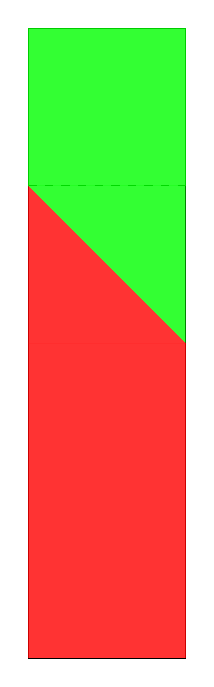
\begin{tikzpicture}[scale=2,transform shape]
    \draw (0,0) rectangle (1,4);
    \draw[dashed] (0,3) -- (1, 3);

    \fill[red, opacity=0.8] (0,0) rectangle (1, 2.001);
    \fill[red, opacity=0.8] (0, 2) -- (1, 2) -- (0, 3) -- cycle;
    \fill[green, opacity=0.8] (1,2) -- (1,3) -- (0,3) -- cycle;
    \fill[green, opacity=0.8] (0, 3) rectangle (1, 4);
  \end{tikzpicture}

  \caption{Top-down representation of a wedge shape in a cubical complex}
  \label{fig:wedge}
\end{figure}

In the figure \ref{fig:wedge}, the red color denotes the cell is covered by a sensor, the green color denotes the cell is free (not covered).
We only allow the object to enter the cell, once it is fully free and can therefore omit the wedge shapes.

The covered planar slices are obtained by performing a union on all the covered areas by all sensors at each point in time.
Covered area is simply a \texttt{Position} representing the top-left corner of a covered cell.

The cubical complex of dimensions $ width \times height \times period $ is constructed by assigning the filtration value of $1$ to free cells and $0$ to covered cells.
According to reasoning described above, a free cell is only free, if it is not covered at 2 consecutive times $t$ and $t + 1$.

\begin{figure}[H]
  \centering
  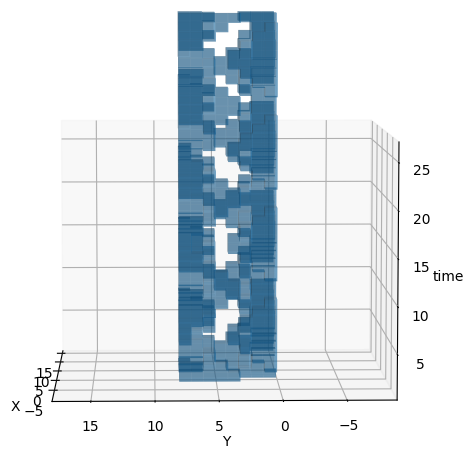
\includegraphics[width=0.7\linewidth]{example_cubical_complex.png}
  \caption{Free cubical complex of the example configuration}
  \label{fig:example_cub_complex}
\end{figure}


\subsection{Computing evasion paths}

Once the cubical complex is obtained, it is collapsed to a directed graph, preserving the homotopy.
The graph is obtained by computing the connected components of the cubical complex at each time (up to period).
Nodes of the graph are of form $(t, label)$, where $t$ is the time and $label$ is the label/index of the connected component.
Each node also holds the data about its \texttt{Position} in the plane, so that we can obtain actual \texttt{Position}s, after computing the cycle.
The edge is added if there exists a non-empty intersection between components at time $t$ and at time $t + 1$.
Note that edges always point in the forward direction of time, therefore any cycle computed on such graph, will always point in the forward direction as well.

\begin{figure}[H]
  \centering
  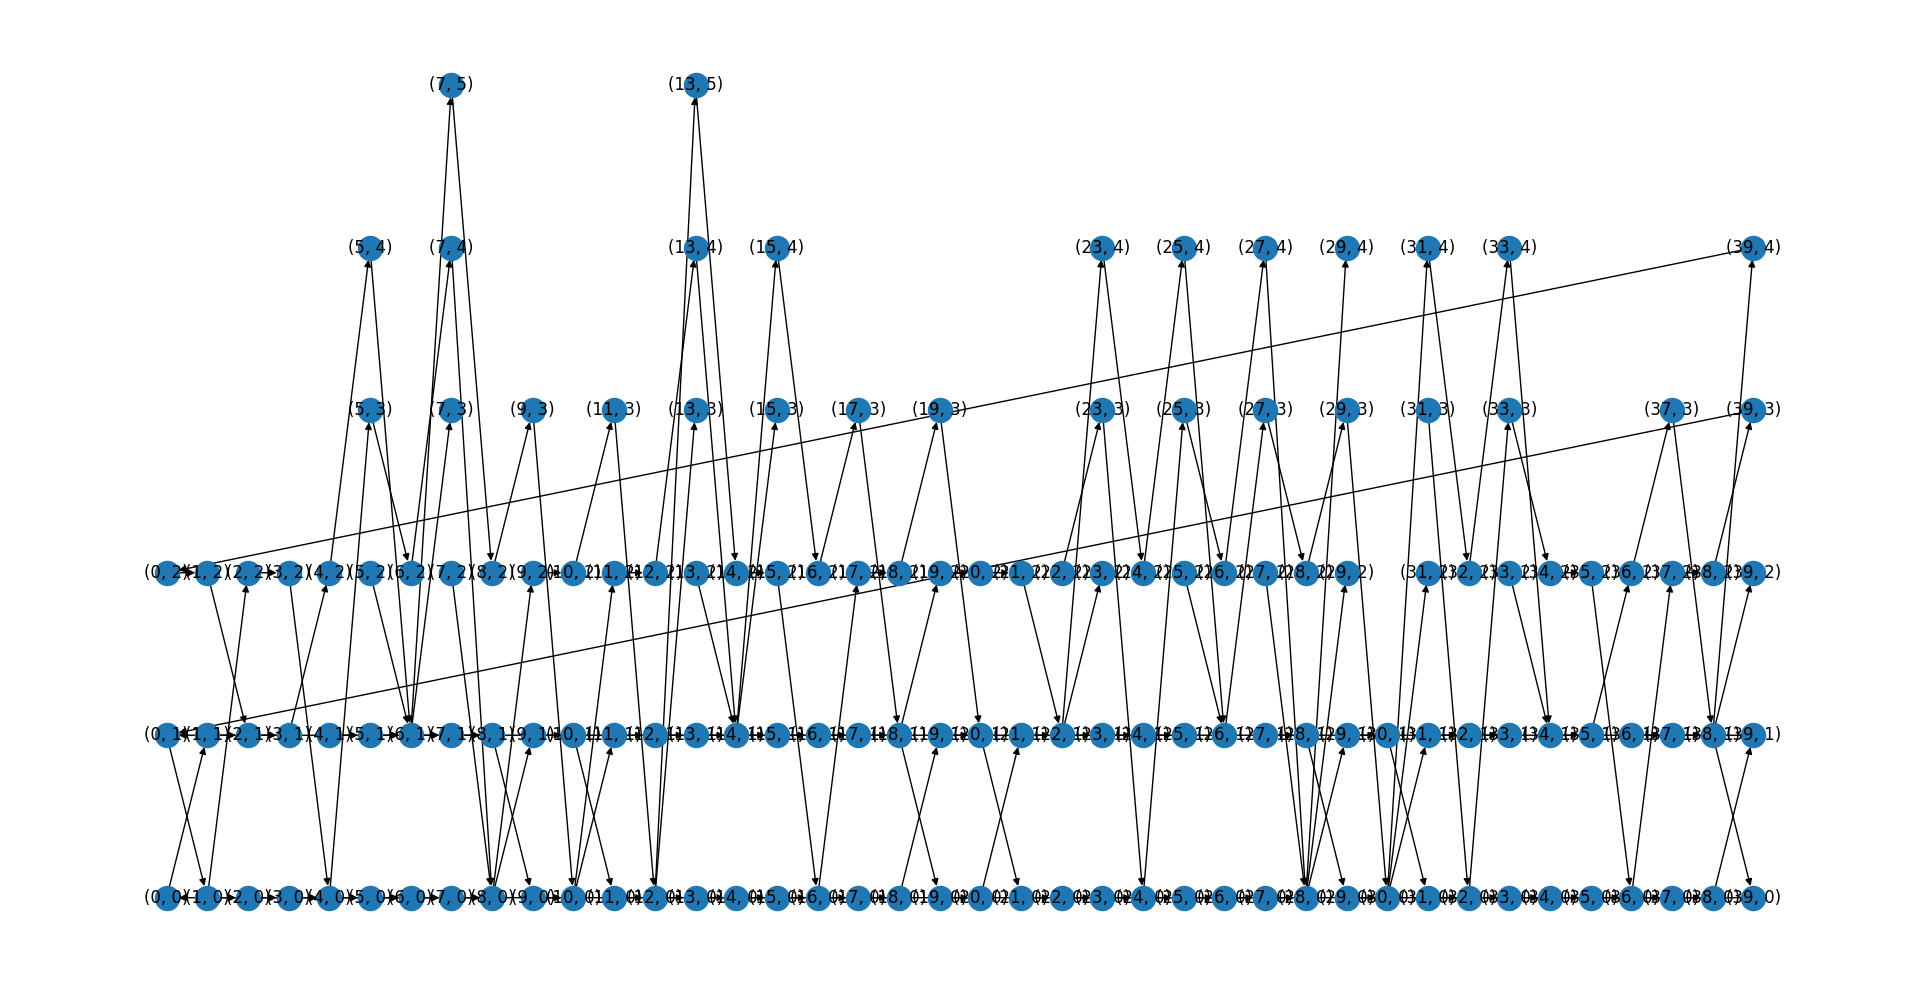
\includegraphics[width=\linewidth]{example_graph.png}
  \caption{Graph of example configuration}
  \label{fig:example_graph}
\end{figure}


Cycles are then obtained by performing a depth first search on the graph and checking whether the current node is equal to the starting node.
Note that, because graph is constructed by only adding the edges in the forward direction, each such cycle will have to loop around the entire complex and will therefore have length equal the period of sensors.


\section{Results}

We tested the algorithm with several configurations.

The first configuration is trivial - a single sensor moving the counter clockwise direction.
\begin{figure}[H]
  \centering
  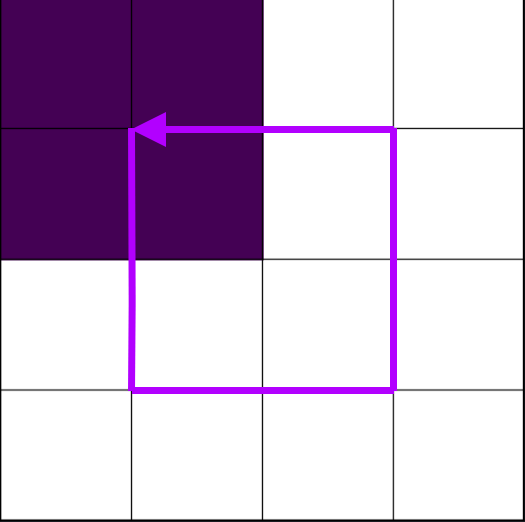
\includegraphics[width=0.7\linewidth]{ccw.png}
  \caption{Counter clockwise circular sensor in 4x4 room, period: 8}
  \label{fig:ccw}
\end{figure}

The algorithm correctly found 1 evasion path.
%TODO: Insert link to gif, once available


\bigskip

The next configuration is the example from the instructions.
\begin{figure}[H]
  \centering
  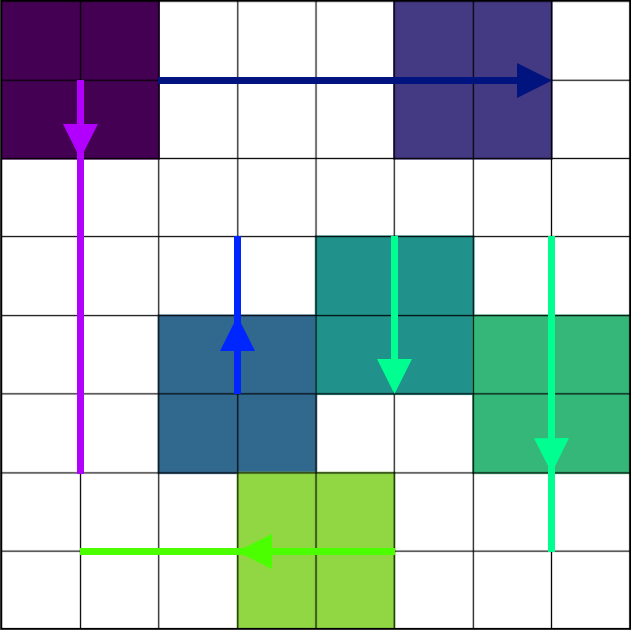
\includegraphics[width=0.7\linewidth]{example.png}
  \caption{6 sensors in 8x8 room, period: 40}
  \label{fig:example}
\end{figure}

Algorithm found 288 evasion paths.
% TODO: Insert link to gif, once available



\section{Discussion}

We implemented evasion path detection by using the Cubical complex structure, reducing it to a graph and finding the cycles there.
This is equivalent to computing the $ H_1(F, \mathbb{Z}) $, on the complex, however this way we did not need to handle edge cases as described.

We also implemented animations of evasion paths, which help to visually confirm whether the algorithm works or not.

Another approach would be to look at a square as 2 adjacent triangles (2-dimensional simplex defined by 3 points), however that would turn out to be more complicated as it would include representing grid-like data with 2 partial segments of it.

A different approach would be to use the zig-zag persistance, which would require us to use the simplicial complexes and also to specify a list of times when each simplex enters and leaves the filtration.


% \section*{Division of work} TODO: Division of work?

% TODO: Bibliography?

\end{document}